\documentclass[border=6pt]{standalone}
\usepackage{tikz}
\usetikzlibrary{arrows.meta,positioning}
\begin{document}
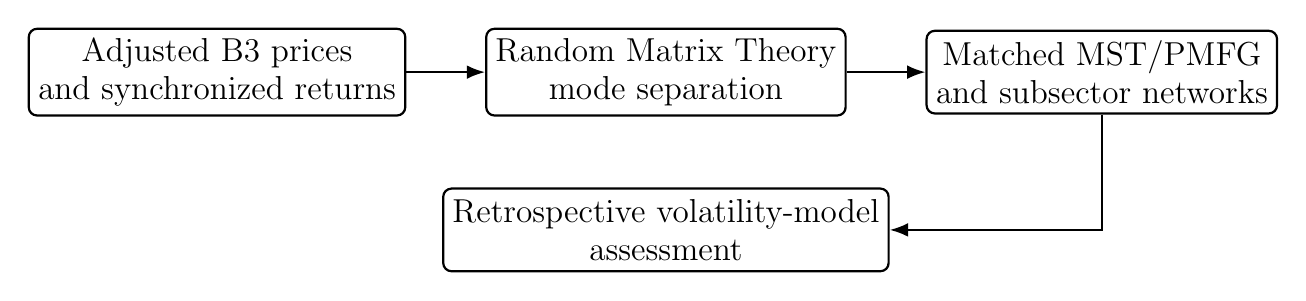
\begin{tikzpicture}[
  >=Latex,
  ga/.style={rectangle, rounded corners=3pt, draw=black, thick,
    align=center, minimum width=4.0cm, minimum height=1.05cm,
    font=\large},
  galine/.style={->, thick}
]
  \node[ga] (data) {Adjusted B3 prices\\and synchronized returns};
  \node[ga, right=1.0cm of data] (rmt) {Random Matrix Theory\\mode separation};
  \node[ga, right=1.0cm of rmt] (net) {Matched MST/PMFG\\and subsector networks};
  \node[ga, below=0.9cm of rmt] (forecast) {Retrospective volatility-model\\assessment};
  \draw[galine] (data) -- (rmt);
  \draw[galine] (rmt) -- (net);
  \draw[galine] (net.south) |- (forecast.east);
\end{tikzpicture}
\end{document}
